\section{Introducción}

Cuando capturamos a través de una cámara una imagen o un vídeo, creamos una representación bidimensional de lo que es en realidad una escena tridimensional. Para conseguir esta reducción de dimensiones, se realiza una proyección de cada uno de los puntos visibles en un plano. Al realizar esta proyección, se pierde una gran cantidad de información relacionada con la profundidad, ya que los puntos ahora representados en el plano bidimensional podían encontrarse a cualquier distancia, siempre y cuando estuviesen situados en la recta que atraviesa el punto verdadero y el centro de la cámara (Figura \ref{fig:proyeccion-perspectiva}).

% TODO: Repasar los finales de línea de esta imagen
\begin{figure}[H]
\centering
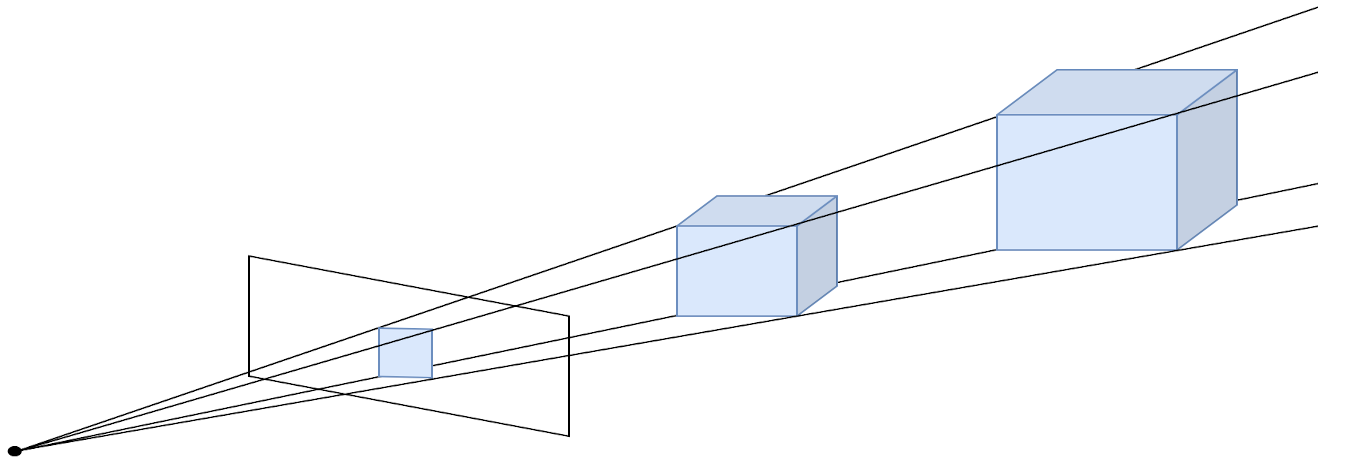
\includegraphics[width=0.65\linewidth]{imagenes/proyeccion-perspectiva.png} 
\captionsetup{width=.8\linewidth}
\caption{Proyección perspectiva y ambigüedad de escala.}
\label{fig:proyeccion-perspectiva}
\end{figure}

Existen soluciones \textit{hardware} que permiten capturar escenas tridimensionales sin perder esta información, por ejemplo: sensores LiDAR, cámaras de tiempo de vuelo, o conjuntos de cámaras para llevar a cabo estereovisión\footnote{Con una pareja de cámaras con posiciones conocidas, es posible estimar la profundidad a partir de la disparidad geométrica entre las dos imágenes capturadas.}\cite{hartley_zisserman_2004}. Sin embargo, estas soluciones requieren de sensores adicionales, con el incremento de material, coste y peso que esto conlleva. Es por esto por lo que recuperar la profundidad (o una estimación de esta) de una imagen obtenida con una cámara corriente sería de gran utilidad, por ejemplo:

\begin{itemize}
    \item En distintas tareas dentro de diferentes campos de aplicación: Navegación robótica y conducción autónoma, empleando la profundidad para reconstruir mapas o calcular el cambio en la posición del agente (odometría visual, VSLAM); detección de superficies y capacidad de incluir oclusión en aplicaciones de realidad aumentada; generación de modelos 3D a través de fotografías (fotogrametría); efectos fotográficos en aplicaciones móviles (efecto \textit{Bokeh}); etc.
    \item Como información adicional o etapa intermedia en otras tareas típicas en visión artificial: detección de objetos, segmentación, clasificación, etc.
\end{itemize}

% https://www.ncbi.nlm.nih.gov/books/NBK11512/
Si observamos, nunca mejor dicho, el sistema visual de los humanos, podemos comprobar como este es un sistema estereoscópico compuesto por dos  ``cámaras''  (los ojos) y un cerebro que interpreta la disparidad entre estas imágenes para obtener una estimación de la profundidad a la que se encuentra cada objeto que vemos. No obstante, si nos tapamos un ojo, aunque con peores resultados, somos capaces de estimar la distancia a la que se encuentran los elementos que están dentro de nuestro campo visual, manteniendo, en una gran mayoría de ocasiones, la capacidad de distinguir cuáles están más cerca y cuáles más lejos. Esto se debe en gran parte a una serie de sesgos cognitivos que los humanos hemos aprendido a medida que crecemos, conocidos como pistas monoculares (pueden ser dinámicas o estáticas, en función de si consideran la información a lo largo del tiempo, por ejemplo, objetos en movimiento), y que no solo se emplean cuando nos tapamos un ojo, si no que también los emplea el cerebro cuando vemos con los dos ojos. Algunas de las principales pistas monoculares (estáticas) \cite{Kalloniatis2005-pc} son: el tamaño relativo con el que observamos un objeto en función de la distancia a la que se encuentre; la oclusión de los elementos que están más próximos que otros; la convergencia de líneas paralelas a medida que se alejan, por ejemplo, en carreteras o vías; el cambio en el tono del color de los objetos lejanos debido a la dispersión de la luz; o la forma de los reflejos y las sombras que producen los elementos, originados por las fuentes de luz de la escena.

No obstante, realizar este análisis de las imágenes monoculares que tan eficientemente llevamos a cabo los humanos en un ordenador de forma automática empleando técnicas de visión artificial tradicional roza lo imposible. Las limitaciones de este tipo de técnicas no solo aparecen en la estimación de profundidades, si no que aparecen en una gran parte de las tareas propias de la visión artificial. Debido a esto, a lo largo de los últimos años se han desarrollado sistemas de aprendizaje automático profundo para trabajar con este tipo de contenido visual, ofreciendo una mucho mayor robustez y capacidad de generalización ante modificaciones en las entradas (cambios de entorno, color, luz, orientación de los elementos, etc.), que suelen ocurrir en los entornos reales, donde es muy difícil controlar dichas variables.

Dentro de estas técnicas, en general, y especialmente para la estimación de profundidades, las redes neuronales convolucionales han prevalecido como las arquitecturas que mejores resultados aportaban. No obstante, en los últimos años han surgido otro tipo de arquitecturas, los \textit{transformers} \cite{NIPS2017_3f5ee243}, que presentan resultados muy competitivos. En vista de esto, este trabajo revisa el estado del arte actual en estimación de profundidad monocular y explora una de las arquitecturas que mejores estimaciones consigue, modificandola para mejorar sus resultados en cuanto al tiempo necesario para inferir la profundidad en una imagen dada. 

\subsection{Motivación}

\todo[inline]{Cambiar este primer párrafo}
La motivación de este trabajo tiene dos partes diferenciadas. En primer lugar, surge la necesidad de estudiar y explorar las distintas técnicas de estimación de profundidades en imagen monocular, tanto sus bases como el estado del arte, para formar una base de conocimiento sobre la que apoyar el desarrollo del resto del trabajo. Este estudio, se plantea como una revisión resumida que pueda ser consultada para facilitar el estudio de las diferentes técnicas existentes, ya que las publicaciones científicas relacionadas con el aprendizaje automático crecen a un ritmo considerablemente difícil de seguir (34736 publicaciones relacionadas con aprendizaje automático en arXiv en el año 2020 \cite{ai_index_report_2021}), lo que denota la utilidad de un documento sobre las distintas arquitecturas y técnicas empleadas en este campo que resuma estos avances y sus características. 

Por otro lado, los modelos del estado del arte son (con excepciones) cada vez más complejos, tienen un mayor número de parámetros, y precisan de grandes cantidades de datos para ser entrenados, lo que conlleva una perdida de accesibilidad al desarrollo y experimentación con dichas arquitecturas, que necesitan una infraestructura costosa para ejecutarse. Además, este incremento en tamaño de los modelos hace que sus velocidades de ejecución e inferencia de resultados se vea afectada. En muchas de las aplicaciones mencionadas en el apartado anterior, el tiempo de inferencia es un factor crítico, ya que muchas veces el procesamiento de las imágenes debe llevarse a cabo en entornos con recursos computacionales limitados y de forma \textit{online}, es decir, procesar las imágenes a medida que están disponibles (sin considerar las restricciones de un entorno de tiempo real). En el caso de que la inferencia de los modelos no se lleve a cabo en dispositivos embebidos y recaiga en servidores a los que los clientes hacen peticiones, un mayor tiempo de ejecución se traduce directamente en un incremento de costes, por lo que tampoco es despreciable. Debido a estas razones, en este trabajo se busca modificar una de los modelos del estado del arte en estimación de profundidades a partir de imágenes monoculares para reducir su tamaño y tiempo de inferencia reduciendo lo mínimo posible la calidad de los resultados.

\subsection{Objetivos}
Los objetivos principales de este Trabajo Fin de Máster, son:
\begin{enumerate}
	\item Llevar a cabo una revisión del estado del arte relacionado con la estimación de profundidades en imágenes monoculares. Más concretamente, en aquellas técnicas que empleen aprendizaje automático, prestando especial atención a las arquitecturas basadas en \textit{transformers}.
    \item Explorar diferentes técnicas generales para acelerar el entrenamiento e inferencia de los modelos de aprendizaje automático profundo. \todo{Checkear esto}
    \item Estudiar una arquitectura del estado del arte de estimación de profundidades y modificar su estructura para acelerar la inferencia y obtener modelos capaces de procesar imágenes de forma \textit{online}, comparando los resultados obtenidos tras ajustar los modelos con distintas variaciones a un \textit{dataset} concreto.
    \item Diseñar una solución en la nube que permita desplegar de forma automática instancias que ejecuten los experimentos necesarios, es decir, entrenando los distintos modelos planteados.
\end{enumerate}


\subsection{Estructura del documento}
\todo[inline]{Redactar}
Introducción; marco teórico y estado del arte; material y métodos; modificaciones de la arquitectura y desarrollo; resultados; discusión; conclusiones y líneas futuras.

\clearpage
